\appendix

\section{Examples of Checks and validations}
\seclabel{ChecksAndValidations}

All the results of the checking and the validation of the program is shown in one integrated view, it is called \emph{Problems}. The figure \figref{problemsview.png} shows a view of this feature. 
There are different types of problems, because these checks and validations are not only used to show type errors or syntax errors, but also to encourage some properties of the program we consider as main topics in the learning process of an OO language.

Here there is a list of all the validations and checking the tool is performing, and a brief reason why they are useful in the teaching of an object oriented language.

Todos los checkeos y problemas
generados se muestran agrupados en una vista dedicada a tal fín (Problems).

\begin{itemize}
  \item \textbf{Syntax Errors}: in this category arises all the errors detected by the parser and the lexical analyser of the language.
  \item \textbf{Style Errors}: this category is useful to teach good practices and to start to talk about code quality, reuse and code sharing.
	\begin{itemize}
		\item \textit{Case in Name}: respecting the difference case conventions for names (\eg using camel case starting with lower case for variables, using camel case starting with upper case for classes).
		\item \textit{Order and grouping}: inside the definition of an object or class the internal references are declared first, then the constructors and finally the methods.
		\item \textit{Modularization}: the classes can only be defined in a library and not in the main program.		
		\item \textit{Duplicated references}: it is impossible to declare a reference using a name already used, this encourage the idea of not having shadowing and improves the readability of the program.
	\end{itemize}
  \item \textbf{References resolution problems}: this errors are useful to detect and avoid references to undeclared variables and also errors in the sending of messages.
  
	\begin{itemize}
	  \item \textit{Undeclared references}: from local variables, parameters or internal fields of objects and classes.
	  \item \textit{Undefined constructors}: checking for the number and type of the parameters.
	  \item \textit{Messages to this}: sending messages to this is a special case, here we can check the existence of the correct method by the number and type of the arguments, even without using type inference.
	\end{itemize}
	
  \item \textbf{Reference usage}: these errors are useful for the detection of erroneous or old code (\eg unused variables or references, sending messages to never assigned variables, using variables instead of values, existence of the overridden method.

  \item \textbf{Type Errors}: the errors are useful for the validation of the compatibility between the references, its possible types, and the messages sent to them, this is performed by the type system and its inferer (\eg message sending, assignation of variables).
\end{itemize}


\section{Implementation}
\label{sec:implementation}
\np{Qué podemos decir de esto}

\section{Images}

	\begin{figure}[p]
	    \centering
		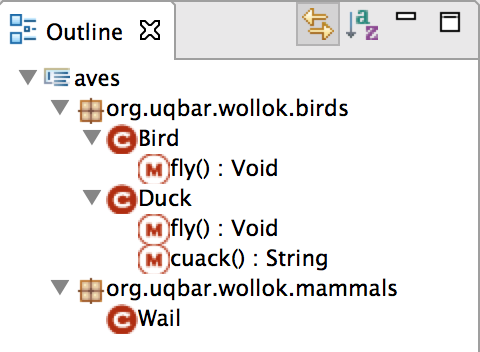
\includegraphics[scale=0.5]{images/wollok-paper-outline.png}
	    \caption{Outline View: This view shows the structure of the file.}
	    \label{fig:outline.png}
	\end{figure}
	
	\begin{figure}[p]
	    \centering
		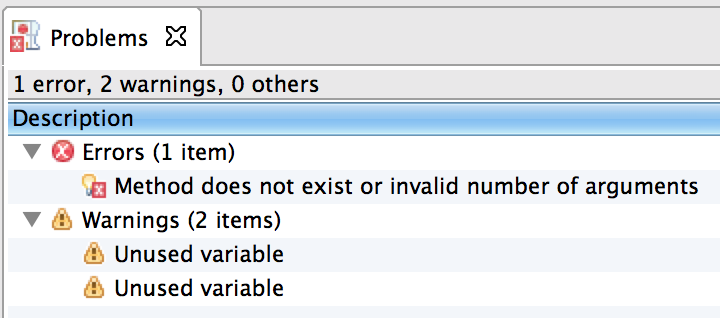
\includegraphics[scale=0.5]{images/wollok-paper-check-problemsview.png}
	    \caption{Problems View: shows the different problems detected by the IDE }
	    \label{fig:problemsview.png}
	\end{figure}
	
	\begin{figure}[p]
	    \centering
		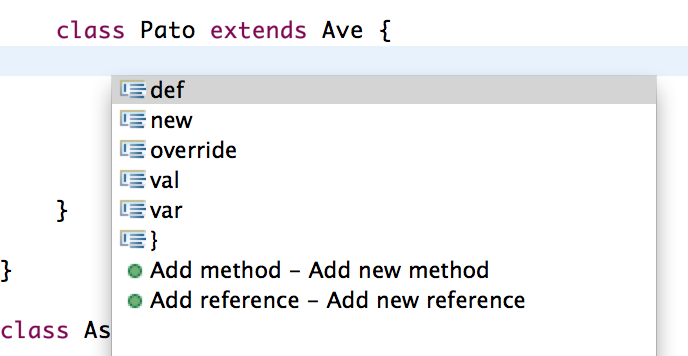
\includegraphics[scale=0.5]{images/wollok-paper-codetemplates.png}
	    \caption{Code Assist: code templates for easy edition}
	    \label{fig:codetemplates.png}
	\end{figure}

	\begin{figure}[p]
	    \centering
		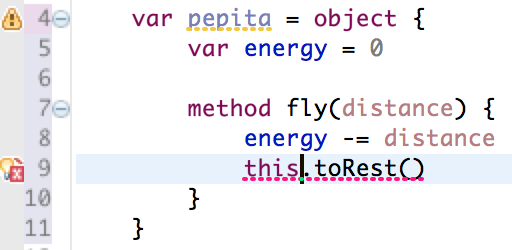
\includegraphics[scale=0.5]{images/wollok-paper-check-noMethodOnThis.png}
	    \caption{Detection of an error on sending a message to \emph{this}}
	    \label{fig:check-noMethodOnThis.png}
	\end{figure}


